\documentclass[12pt]{scrartcl}

\setlength{\parindent}{0pt}
\setlength{\parskip}{.25cm}

\usepackage{graphicx}

\usepackage{xcolor}

\definecolor{darkred}{rgb}{0.5,0,0}
\definecolor{darkgreen}{rgb}{0,0.5,0}
\usepackage{hyperref}
\hypersetup{
  letterpaper,
  colorlinks,
  linkcolor=red,
  citecolor=darkgreen,
  menucolor=darkred,
  urlcolor=blue,
  pdfpagemode=none,
  pdftitle={CSCE 156 Lab Handout},
  pdfauthor={Christopher M. Bourke},
  pdfsubject={},
  pdfkeywords={}
}

\definecolor{MyDarkBlue}{rgb}{0,0.08,0.45}
\definecolor{MyDarkRed}{rgb}{0.45,0.08,0}
\definecolor{MyDarkGreen}{rgb}{0.08,0.45,0.08}

\definecolor{mintedBackground}{rgb}{0.95,0.95,0.95}
\definecolor{mintedInlineBackground}{rgb}{.90,.90,1}

%\usepackage{newfloat}
\usepackage[newfloat=true]{minted}
\setminted{mathescape,
               linenos,
               autogobble,
               frame=none,
               framesep=2mm,
               framerule=0.4pt,
               %label=foo,
               xleftmargin=2em,
               xrightmargin=0em,
               startinline=true,  %PHP only, allow it to omit the PHP Tags *** with this option, variables using dollar sign in comments are treated as latex math
               numbersep=10pt, %gap between line numbers and start of line
               style=default, %syntax highlighting style, default is "default"
               			    %gallery: http://help.farbox.com/pygments.html
			    	    %list available: pygmentize -L styles
               bgcolor=mintedBackground} %prevents breaking across pages
               
\setmintedinline{bgcolor={mintedBackground}}
\setminted[text]{bgcolor={mintedBackground},linenos=false,autogobble,xleftmargin=1em}
%\setminted[php]{bgcolor=mintedBackgroundPHP} %startinline=True}
\SetupFloatingEnvironment{listing}{name=Code Sample}
\SetupFloatingEnvironment{listing}{listname=List of Code Samples}

\title{CSCE 156 -- Computer Science II}
\subtitle{Lab 7.0 - SQL I}
\author{~}
\date{~}

\begin{document}

\maketitle

\section*{Prior to Lab}

\begin{enumerate}
  \item Review this laboratory handout prior to lab.
  \item Create a MySQL account by logging in here: \url{https://cse-apps.unl.edu/amu/login}
  \item Change the account password using the following directions at: 
  	\url{http://cse.unl.edu/faq-section/unix-linux#node-302}
  \item Review the supplemental SQL Cheat Sheet for the Album Database
  \item This is a long lab but it can be completed if you prepare 
	properly.  Review the following materials:
  \begin{itemize}
    \item Information About Databases and Tables \\
    \url{http://dev.mysql.com/doc/refman/5.6/en/getting-information.html}
    \item Connecting to MySQL from the command line: \\ 
    \url{http://dev.mysql.com/doc/refman/5.6/en/connecting-disconnecting.html}
    \item Retrieving data\\ \url{http://www.w3schools.com/sql/sql_select.asp}
    \item Conditional clause	\\ \url{http://www.w3schools.com/sql/sql_where.asp} 
    \item Inserting data	\\ \url{http://www.w3schools.com/sql/sql_insert.asp} 
    \item Deleting data	\\ 
    \url{http://www.w3schools.com/sql/sql_delete.asp} 
    \item Updating data	\\ 
    \url{http://www.w3schools.com/sql/sql_update.asp} 
    \item \mintinline{sql}{count()}	\\ 
    \url{http://www.w3schools.com/sql/sql_func_count.asp}
    \item \mintinline{sql}{max()}	\\ \url{http://www.w3schools.com/sql/sql_func_max.asp}
    \item \mintinline{sql}{min()}	\\ \url{http://www.w3schools.com/sql/sql_func_min.asp}
    \item Joining tables	inner join	\\ 
    \url{http://www.w3schools.com/sql/sql_join_inner.asp} 
	\item left join	\\ 
    \url{http://www.w3schools.com/sql/sql_join_left.asp} 
	\item right join	\\ 
    \url{http://www.w3schools.com/sql/sql_join_right.asp} 
  \end{itemize}  
\end{enumerate}

\section*{Lab Objectives \& Topics}
Following the lab, you should be able to:
\begin{itemize}
  \item Connect to a database and execute queries
  \item Perform basic Create, retrieve, update, and delete (CRUD) operations
  \item Understand more complex queries using Joins and Aggregate functions
\end{itemize}

\section*{Peer Programming Pair-Up}

To encourage collaboration and a team environment, labs will be
structured in a \emph{pair programming} setup.  At the start of
each lab, you will be randomly paired up with another student 
(conflicts such as absences will be dealt with by the lab instructor).
One of you will be designated the \emph{driver} and the other
the \emph{navigator}.  

The navigator will be responsible for reading the instructions and
telling the driver what to do next.  The driver will be in charge of the
keyboard and workstation.  Both driver and navigator are responsible
for suggesting fixes and solutions together.  Neither the navigator
nor the driver is ``in charge.''  Beyond your immediate pairing, you
are encouraged to help and interact and with other pairs in the lab.

Each week you should alternate: if you were a driver last week, 
be a navigator next, etc.  Resolve any issues (you were both drivers
last week) within your pair.  Ask the lab instructor to resolve issues
only when you cannot come to a consensus.  

Because of the peer programming setup of labs, it is absolutely 
essential that you complete any pre-lab activities and familiarize
yourself with the handouts prior to coming to lab.  Failure to do
so will negatively impact your ability to collaborate and work with 
others which may mean that you will not be able to complete the
lab.  

\section*{Getting Started}

Material for this lab is available for download on the course website.

\section*{Querying a Database}

You will be connecting to a remote MySQL database server on CSE 
and executing several queries.  The queries you will be performing 
involve a database that contains data about various music albums, songs
and the artists involved.  The database structure is illustrated 
in the ER (Entity-Relation) diagram in Figure \ref{figure:albumDB}.

\begin{figure}[h]
\centering
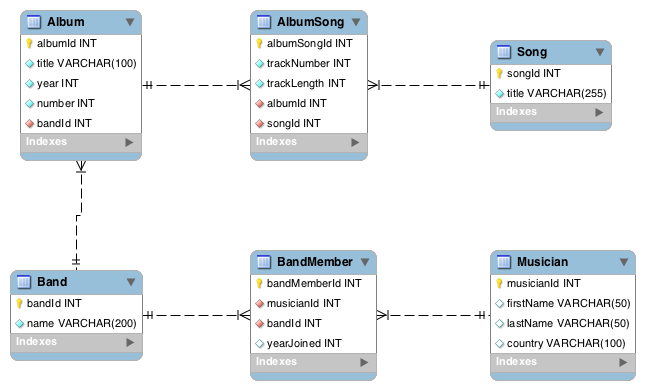
\includegraphics[scale=.650]{sql/albums}
\caption{Albums Database}
\label{figure:albumDB}
\end{figure}

\subsection*{Importing the Database}

You will need to ``install'' the Albums database and data into your 
own database on CSE.  Note: ``database'' in this sense is just a collection 
of related tables; on CSE you only have access to one actual 
database--the database named after your CSE login.  

\subsubsection*{Using MySQL Workbench}

To install using MySQL Workbench, change the \mintinline{sql}{use LOGIN;}
line to use your own login and then cut-paste the entire script into MySQL
Workbench and run it.  

\subsubsection*{Using The Command Line}

To install from the command line change the \mintinline{sql}{use LOGIN;}
line to use your own login and then:

\begin{enumerate}
  \item Make sure the \mintinline{text}{albums.sql} DDL file (Data 
  	Description Language) is on your Z drive.  
  \item From the command line (via PuTTY), execute the following:
  
  \mintinline{text}{mysql -u username -p username < albums.sql}
  
  where \mintinline{text}{username} is replaced with your CSE login.
  Enter your MySQL password.  This redirects the contents of the 
  \mintinline{text}{albums.sql} file (a collection of SQL commands) 
  to the mysql command line interface, creating all the tables and 
  inserting all the data necessary.
\end{enumerate}
  
\subsection*{Executing Queries}

You may use any interface to your MySQL database that you wish, but 
we recommend that you use MySQL Workbench.  You can download and
install it from here: \url{https://www.mysql.com/products/workbench/}.
Otherwise, it is available on the CSE lab computers.

\begin{enumerate}
  \item Launch MySQL Workbench
  \item From the quick launch menu select ``Open Connection to Start Querying''
  \item Enter the host name (cse.unl.edu), username (your cse login) 
    and enter your sql password; click ``OK''
  \item You can now enter queries and execute them (follow the menu options)
\end{enumerate}

Execute the queries in the worksheet and demonstrate them to a
lab instructor.  Instead of writing the answers by hand, you may
simply type them in the worksheet provided.
  
\subsection*{SQL Supplemental Cheat Sheet}

For your benefit, we have created a supplemental SQL cheat sheet that 
you may reference.  It contains many of the major types of queries 
along with a practical application using the Album database.

\end{document}
